\chapter{Virt-manager}
\section{Pré-requis et considérations pour les hôtes}
Divers facteurs doivent être considérés avant de créer des hôtes virtualisés.
\subsubsection{Performance} 
Les hôtes virtualisés doivent être déployés et configurés en fonction de leurs tâches prévues. Certains systèmes (par exemple, les hôtes où sont hébergés des serveur de base de données) ont besoin de performances plus élevées que d'habitude. Les hôtes peuvent exiger plus de CPU ou de mémoire attribué en fonction de leur rôle et de l'utilisation future qu'il pourrait avoir.
\subsubsection{Stockage}
Certains hôtes peuvent avoir besoin d'une plus grande priorité d'accès au stockage, de disques plus rapides, ou peuvent exiger un accès exclusif à des zones de stockage. La quantité de stockage utilisée par les hôtes doit être régulièrement surveillée et prise en compte lors du déploiement et le maintien de stockage.
\subsubsection{Mise en réseau et l'infrastructure du réseau}
 En fonction de notre environnement, certains hôtes pourraient exiger des liens réseaux plus rapides que d'autres hôtes. La bande passante ou de latence sont souvent des facteurs à prendre en compte lors du déploiement et la maintenance des hôtes.
\section{Installation côté serveur}
Cette partie est facile, un simple apt-get install suffit. Nous installons le paquet qui communique avec Xen et remonte les informations au client virt-manager.
\begin{lstlisting}
apt-get install libvirt-bin
\end{lstlisting} 
Du coté de Xen, nous devons vérifier qu’il peut communiquer avec libvirt.

Libvirt accède aux données de Xen via un socket unix. La configuration consiste à activer cette option dans Xen et à relancer les services.
Nous éviterons ainsi l’erreur \emph{libvirtError: internal error failed to connect to xend} dont on trouve peu d’explication sur le net.
\\
Un autre bug rencontré nécessite la correction d'un lien symbolique et l'installation de qemu.

\begin{lstlisting}
# Installation de qemu-dm pour créer des machines virtuelles en mode full virtualisé
apt-get install xen-qemu-dm-4.0 -y

# Correction d'un bug de qemu qui invalidait un lien symbolique
mkdir /usr/lib64/xen
mkdir /usr/lib64/xen/bin
cd /usr/lib64/xen/bin
ln -s /usr/lib/xen-4.0/bin/qemu-dm
\end{lstlisting} 

On édite le fichier de configuration xen
\begin{lstlisting} 
nano /etc/xen/xend-config.sxp
\end{lstlisting}
 on active, ou on rajoute la ligne suivante
\begin{lstlisting} 
(xend-unix-server yes)
\end{lstlisting}
 Enfin on relance le service xen avec /etc/init.d/xend restart

\section{Installation côté client}
Pour gérer nos serveurs, nous installons virt-manager avec la commande suivante:
\begin{lstlisting} 
apt-get install virt-manager
\end{lstlisting}
Au premier lancement, seule la connexion locale est active. Pour ajouter un nouveau noeud, on peut passer par le menu \emph{File>Add Connection} auquel cas il faut modifier le type pour le positionner sur \emph{xen+ssh} et renseigner le nom du noeud.
\begin{center}
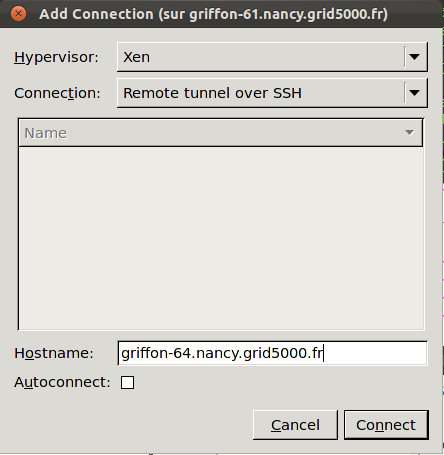
\includegraphics[width=250pt]{images/nouvelle_conn.png}
\end{center}
Virt-manager étant un outil graphique, ses fichiers de configurations sont gérés par gconf. Ainsi, pour automatiser l'ajout des différents noeuds nous avons crée un script qui réécrit le fichier \emph{~/.gconf/apps/virt-manager/connections/\%gconf.xml}
\begin{lstlisting}
for node in $(cat $list_nodes)
do
    echo '<li type="string">' >> $fichier
    echo "<stringvalue>xen+ssh://root@$node/</stringvalue>" >> $fichier
    echo '</li>' >> $fichier
done
\end{lstlisting}
Ce fichier est au format xml et contient pour chaque noeud une entrée. Ici, les connexions sont gérées au-dessus d'un tunnel ssh. Commme nous ne pouvions pas accéder depuis l'extérieur, aux noeuds de Grid5000, nous avons dû installer virt sur les noeuds eux-mêmes (qui sont donc à la fois clients et serveurs) et y accéder via le X Forwarding de la connexion ssh.
\section{Création d'hôtes virtualisés avec virt-manager}
Pour commencer, on démarre virt-manager, puis on lance le gestionnaire de machines virtuelles à partir du menu en cliquant sur l'icone en forme de pc.

%\begin{figure}
\begin{center}
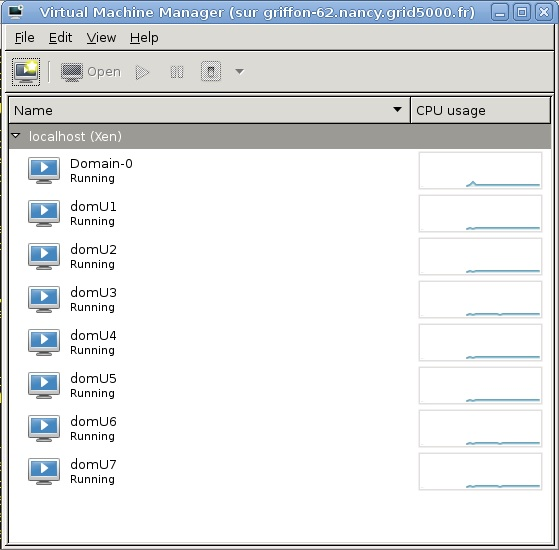
\includegraphics[width=350pt]{images/virt.jpg}
\end{center}
%\caption{Interface de virt-manager}
%\end{figure}

La fenêtre du gestionnaire de machine virtuelle nous autorise à en créer de nouvelles.\\
On clique sur création de nouvelle machine virtuelle pour faire apparaître l'assistant qui va nous aider pour élaborer notre hôte.
L'assistant décompose la création en cinq étapes:
\begin{itemize}
\item La localisation et la configuration des supports d'installation.
\item La configuration de la mémoire et les options de CPU.
\item La configuration du stockage de l'invité.
\item La configuration réseau, l'architecture, et d'autres paramètres matériels.
\end{itemize}
Le processus de création d'hôte commence avec la sélection d'un nom et le type d'installation.

\subsubsection{Localisation et Configuration des supports d'installation.}
%\begin{figure}
\begin{center}
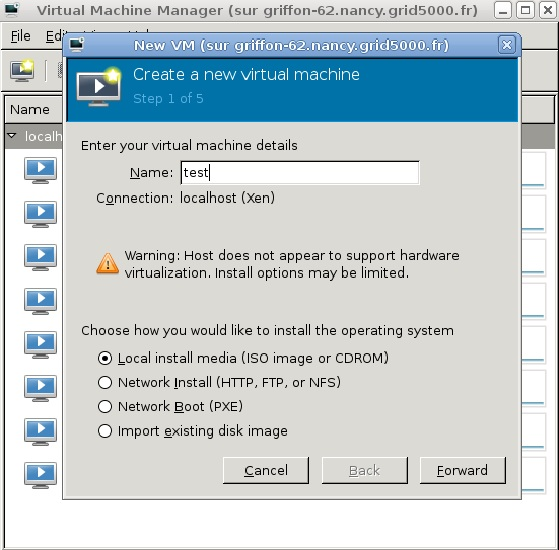
\includegraphics[width=350pt]{images/nommachine.jpg}
\end{center}
%\caption{Choix du nom de la nouvelle machine virtuelle}
%\end{figure}
\begin{description}
  \item[Local install media(ISO image or CDROM) :] Cette méthode utilise un CD-ROM,DVD ou une image iso.
  \item[Network install :] Cette méthode utilise le réseau pour installer le système d'exploitation.
  \item[Network Boot :] Ceci permet de résupérer un environement exécutable directement depuis le réseau et donc sans installation nécessaire.
  \item[Import existing disk image :] Cette méthode nous permet de créer un nouvelle hôte et d'y importer une image disque.
\end{description}
La prochaine étape consiste à configurer l'installation.\\
On configure le type de système d'exploitation et sa version qui sera installée, cela dépend de la méthode d'installation que l'on a choisi.
%\begin{figure}
\begin{center}
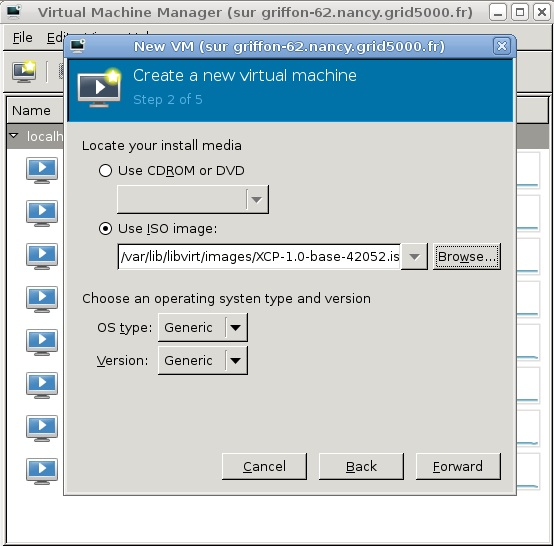
\includegraphics[width=300pt]{images/iso.jpg}
\end{center}
%\caption{Choix du nom de la nouvelle machine virtuelle}
%\end{figure}

\subsubsection{Configuration du CPU et de la mémoire}
La prochaine étape consiste à configurer le nombre de CPU et la quantité de mémoire à allouer à la machine virtuelle. L'assistant indique le nombre de processeurs et la quantité de mémoire que l'on peut lui allouer.
%\begin{figure}
\begin{center}
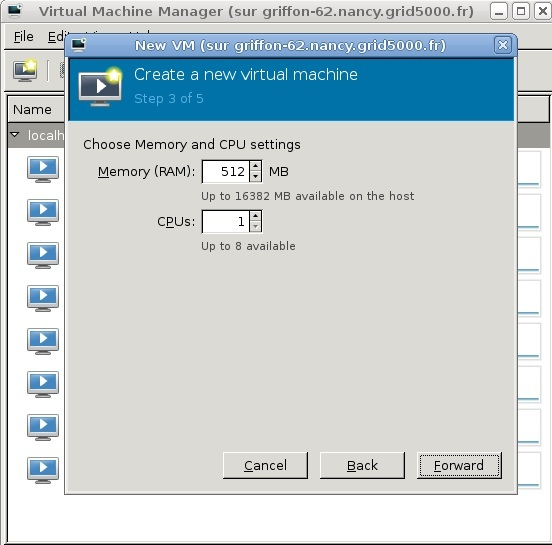
\includegraphics[width=300pt]{images/cpu.jpg}
\end{center}
%\caption{Configuration du CPU et de la mémoire allouée à la machine virtuelle}
%\end{figure}

\subsubsection{Configuration de l'espace de stockage}
%\begin{figure}
\begin{center}
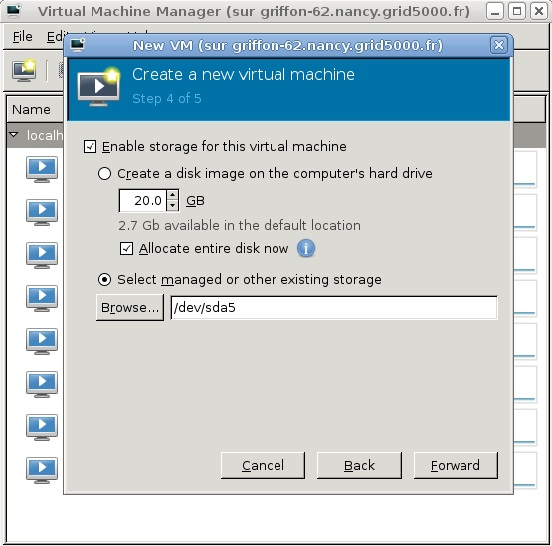
\includegraphics[width=300pt]{images/Storage.jpg}
\end{center}
%\caption{Choix du stockage de la machine virtuelle}
%\end{figure}

 Si l'on a choisi d'importer une image de disque existante au cours de la première étape, virt-manager va sauter cette étape.
On doit attribuer un espace suffisant pour notre machine virtuelle et toutes les applications que l'hôte a besoin.

\subsubsection{ Configuration réseau et architecture}
On vérifie les paramètres de la machine virtuelle et on clique sur Terminer lorsqu'on est satisfait, cela permettra de créer l'hôte avec les paramètres réseaux par défaut, le type de virtualisation, et l'architecture.
\begin{center}
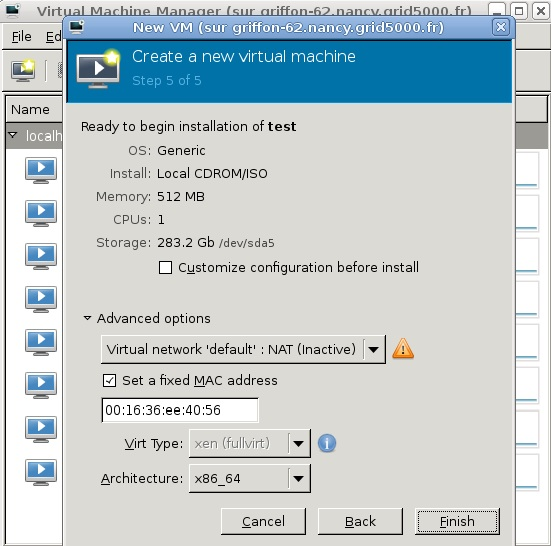
\includegraphics[width=300pt]{images/reseau.jpg}
\end{center}
%\caption{Configuration du réseau}


\subsection{Controle d'hotes distants}
On peut facilement manager des hotes distants une fois ceux-ci enregistrés dans virt-manager. Cette opération peut être fastidieuse car virt étant un programme graphique, créer un script pour automatiser l'ajout de plusieurs dizaines de noeuds s'est avéré plus compliqué que prévu.
Cherchant désespérément un fichier de configuration, nous avons fini par le trouver en lançant une recherche dans tout le système sur les noms des noeuds ajoutés à virt. Le fichier est donc géré par \emph{gconf} en voici un exemple
\lstinputlisting[language=xml,morekeywords={li,entry,stringvalue,gconf},caption={Fichier .gconf/apps/virt-manager/connections/\%gconf.xml}]{scripts/virt-manager/gconf.xml}
Après l'installation de virt, le seul lien enregistré est le lien local. Pour ajouter une connexion vers un nouvel hote xen, on peut utiliser l'interface graphique.
%\includegraphics image ajout d'un noeud
Cependant, dans notre cas, il était assez fastidieux de renseigner manuellement chacun des noeuds surtout lors des tests à grande échelle. C'est pourquoi nous avons fait un script (voir annexe \ref{ajout-noeuds} en page \pageref{ajout-noeuds}) donc voici la boucle d'ajout des noeuds:
\begin{lstlisting}[language=bash]
#Pour chaque noeud réservé, on ajoute une entrée dans le fichier
for node in $(cat $list_nodes)
do
    echo '<li type="string">' >> $fichier
    echo "<stringvalue>xen+ssh://root@$node/</stringvalue>" >> $fichier
    echo '</li>' >> $fichier
done
\end{lstlisting}
Le script de base ayant configuré chacun des noeuds de la même manière, ils peuvent tous être utilisés pour gérer l'ensemble du réseau, une fois le script exécuté.
\begin{center}
  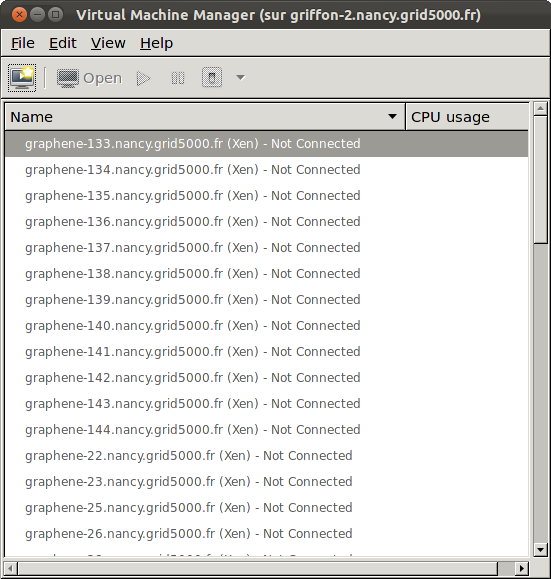
\includegraphics[width=300pt]{images/virt-ajout_noeuds.png}
\end{center}
Un simple clic sur un noeud établit la connexion puisque les mêmes clés ssh ont été copiées partout et le fichier \emph{known\_hosts} a également été répliqué pour éviter de confirmer l'ajout d'un hôte inconnu (opération qui devait se faire en ligne de commande car non gérée par virt).
\\
On est ensuite en mesure de créer une machine sur n'importe quel noeud, la procédure étant la même que pour une installation locale, nous n'allons pas la détailler à nouveau.

\subsection{Migration de machines}
Une fonctionnalité intéressante d'un gestionnaire de machines virtuelles est la migration des systèmes invités vers un autre hôte pour prévoir des opérations de maintenance, remplacement,...\\
Encore une fois virt-manger possède un outil graphique afin d'assister cette étape. Pour commencer, en effectuant un click droit sur une machine virtuelle on obtient un menu contextuel que nous allons détaillé au fur et à mesure.
\begin{center}
  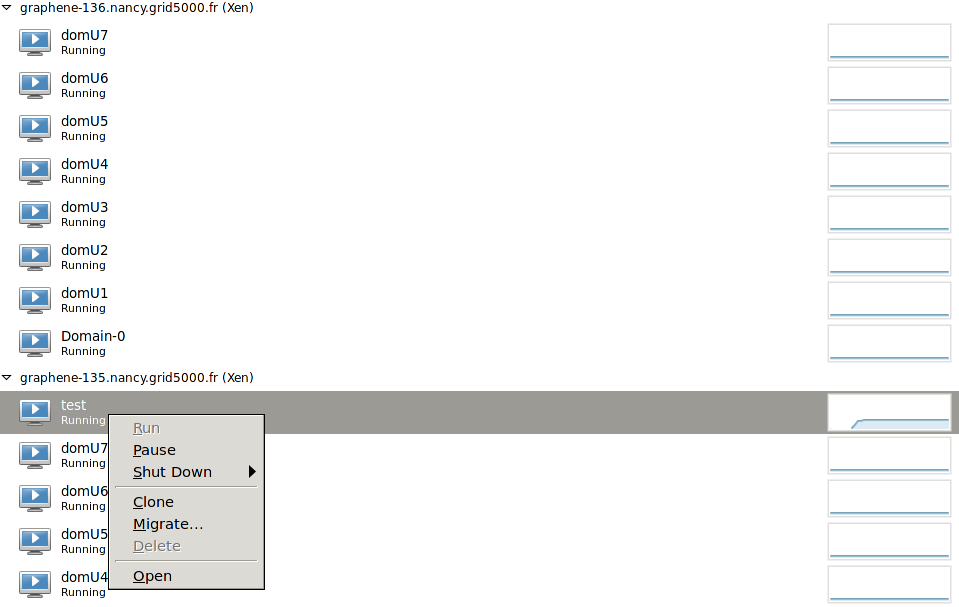
\includegraphics[width=350pt]{images/virt-menu-context.png}
\end{center}
En sélectionnant l'option \emph{Migrate} l'assistant demande alors sur quel autre noeud (préalablement ajouté à virt) nous souhaitons transférer la machine virtuelle. L'opération peut prendre plusieures minutes en fonctions des capacités des machines et du réseau.
\begin{center}
  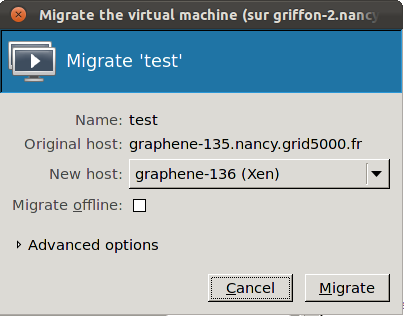
\includegraphics[width=250pt]{images/migration1.png}
\end{center}
\begin{center}
  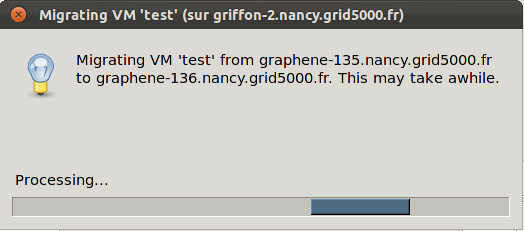
\includegraphics[width=250pt]{images/migration.png}
\end{center}
